\documentclass[12pt]{article}
\setlength{\oddsidemargin}{0in}
\setlength{\evensidemargin}{0in}
\setlength{\textwidth}{6.5in}
\setlength{\parindent}{0in}
\setlength{\parskip}{\baselineskip}
\usepackage{amsmath,amsfonts,amssymb}
\usepackage{graphicx}
\usepackage{enumitem}
\usepackage[]{algorithmicx}
\usepackage{amsthm}
\usepackage{fancyhdr}
\pagestyle{fancy}
\setlength{\headsep}{36pt}
\usepackage{tkz-berge}
\usetikzlibrary{positioning, automata}

\usepackage{hyperref}

\theoremstyle{remark}
\newtheorem*{solution}{Solution}

\newcommand{\makenonemptybox}[2]{%
%\par\nobreak\vspace{\ht\strutbox}\noindent
\item[]
\fbox{% added -2\fboxrule to specified width to avoid overfull hboxes
% and removed the -2\fboxsep from height specification (image not updated)
% because in MWE 2cm is should be height of contents excluding sep and frame
\parbox[c][#1][t]{\dimexpr\linewidth-2\fboxsep-2\fboxrule}{
  \hrule width \hsize height 0pt
  #2
 }%
}%
\par\vspace{\ht\strutbox}
}
\makeatother

\begin{document}
\definecolor {processblue}{cmyk}{0.96,0,0,0}

\lhead{{\bf CSCI 3104, Algorithms \\ Problem Set 5b (48 points)} }
\rhead{Name: \fbox{Michael Rogers} \\ ID: \fbox{105667404} \\ {\bf Profs.\ Hoenigman \& Agrawal\\ Fall 2019, CU-Boulder}}
\renewcommand{\headrulewidth}{0.5pt}

\phantom{Test}

\begin{small}
\textbf{Instructions for submitting your solution}:
\vspace{-5mm} 

\begin{itemize}
	\item The solutions \textbf{should be typed} and we cannot accept hand-written solutions. \href{http://ece.uprm.edu/~caceros/latex/introduction.pdf}{Here's a short intro to Latex.}
	\item You should submit your work through \href{https://www.gradescope.com/courses/59294}{\textbf{Gradescope}} only.
	\item If you don't have an account on it, sign up for one using your CU email. You should have gotten an email to sign up. If your name based CU email doesn't work, try the identikey@colorado.edu version. 
	\item Gradescope will only accept \textbf{.pdf} files (except for code files that should be submitted separately on Gradescope if a problem set has them) and \textbf{try to fit your work in the box provided}. 
	\item You cannot submit a pdf which has less pages than what we provided you as Gradescope won't allow it. 
	\item Verbal reasoning is typically insufficient for full credit. Instead, write a logical argument, in the style of a mathematical proof.
	\item For every problem in this class, you must justify your answer:\ show how you arrived at it and why it is correct. If there are assumptions you need to make along the way, state those clearly.
	
	\item You may work with other students. However, \textbf{all solutions must be written independently and in your own words.} Referencing solutions of any sort is strictly prohibited. You must explicitly cite any sources, as well as any collaborators. 
\end{itemize}



\vspace{-4mm} 
\end{small}

\hrulefill

\newpage
\begin{enumerate}

\item (25 pts) For this question, you are going to implement Kruskal's algorithm and union-find to build an MST from supplied data. Refer to the python starter code \\ \textbf{MST\_Q1\_starter\_code.py} on Canvas that generates a graph of US cities, where the cities are the vertices and the edges are the distances between them. The code requires \textbf{miles\_dat.txt.gz} file as the graph data source so keep it in the same folder as the code. Before you start writing any code, make sure you can build the code that's been supplied. The code uses the networkx library. You may need to install this library for the code to run.

\textbf{Read all instructions for this question carefully.} 

\begin{enumerate}[label=(\alph*)]

\item (5 pts) Complete the code to find the edges that are part of the MST. You should add these edges in the list $kruskal\_selected\_edges$. Do not change the existing format of the edges. They are represented as a tuple of vertices and a vertex is represented like $v = \text{"Waukegan, IL"}$. Read the comments in the code for more information. You don't need to read/understand the $miles\_graph()$ and $draw\_graph()$ functions. 

\item (10 pts) Implement the $union()$ function to implement Kruskal's.\\


\item (10 pts) Modify your code slightly so that you can produce disconnected components. Let's call these components clusters. The “spacing” of any particular clustering (group of clusters) is defined as the smallest edge between vertices in any pair of different clusters. If we stop Kruskal's $k$ iterations before the algorithm completes, what is the spacing value? Run your code for $k = 2...10$ to generate spacing for all these k values. Your code needs to have this calculation for your answer to receive credit. \\
\item In the pdf that you submit for this assignment, please include the following:
\begin{enumerate}
    \item One of the generated graphs \textbf{MST.png} that your code produces that shows the MST for that run. Note that on each run, you can get a different number of edges to begin with. Thus, you can expect a different answer each time you run.
    \item The spacing values for each $k$ value that you use.
    \item Your .py file for this question needs to be submitted to Canvas.
\end{enumerate}
\pagebreak

(Space for Q1 image and spacing values)
\pagebreak


\end{enumerate}

\item (3 pts) How many disconnected components are there when you stop Kruskal's $k$ round before you complete the MST? Justify your answer. 
\begin{solution}

\end{solution}


\item (5 pts) Consider the recurrence $F_{n} = 2F_{n-1} + F_{n-2}$, with the base cases $F_{0} = 1$ and $F_{1} = 2$. Suppose we have letters $v_{0}, \ldots, v_{7}$; where for $i \in \{0, \ldots, 7\}$, the frequency of $v_{i}$ is given by $F_{i}$. Draw a Huffman tree for $v_{0}, \ldots, v_{7}$. 

\begin{solution}Drawing of Huffman Tree: \\
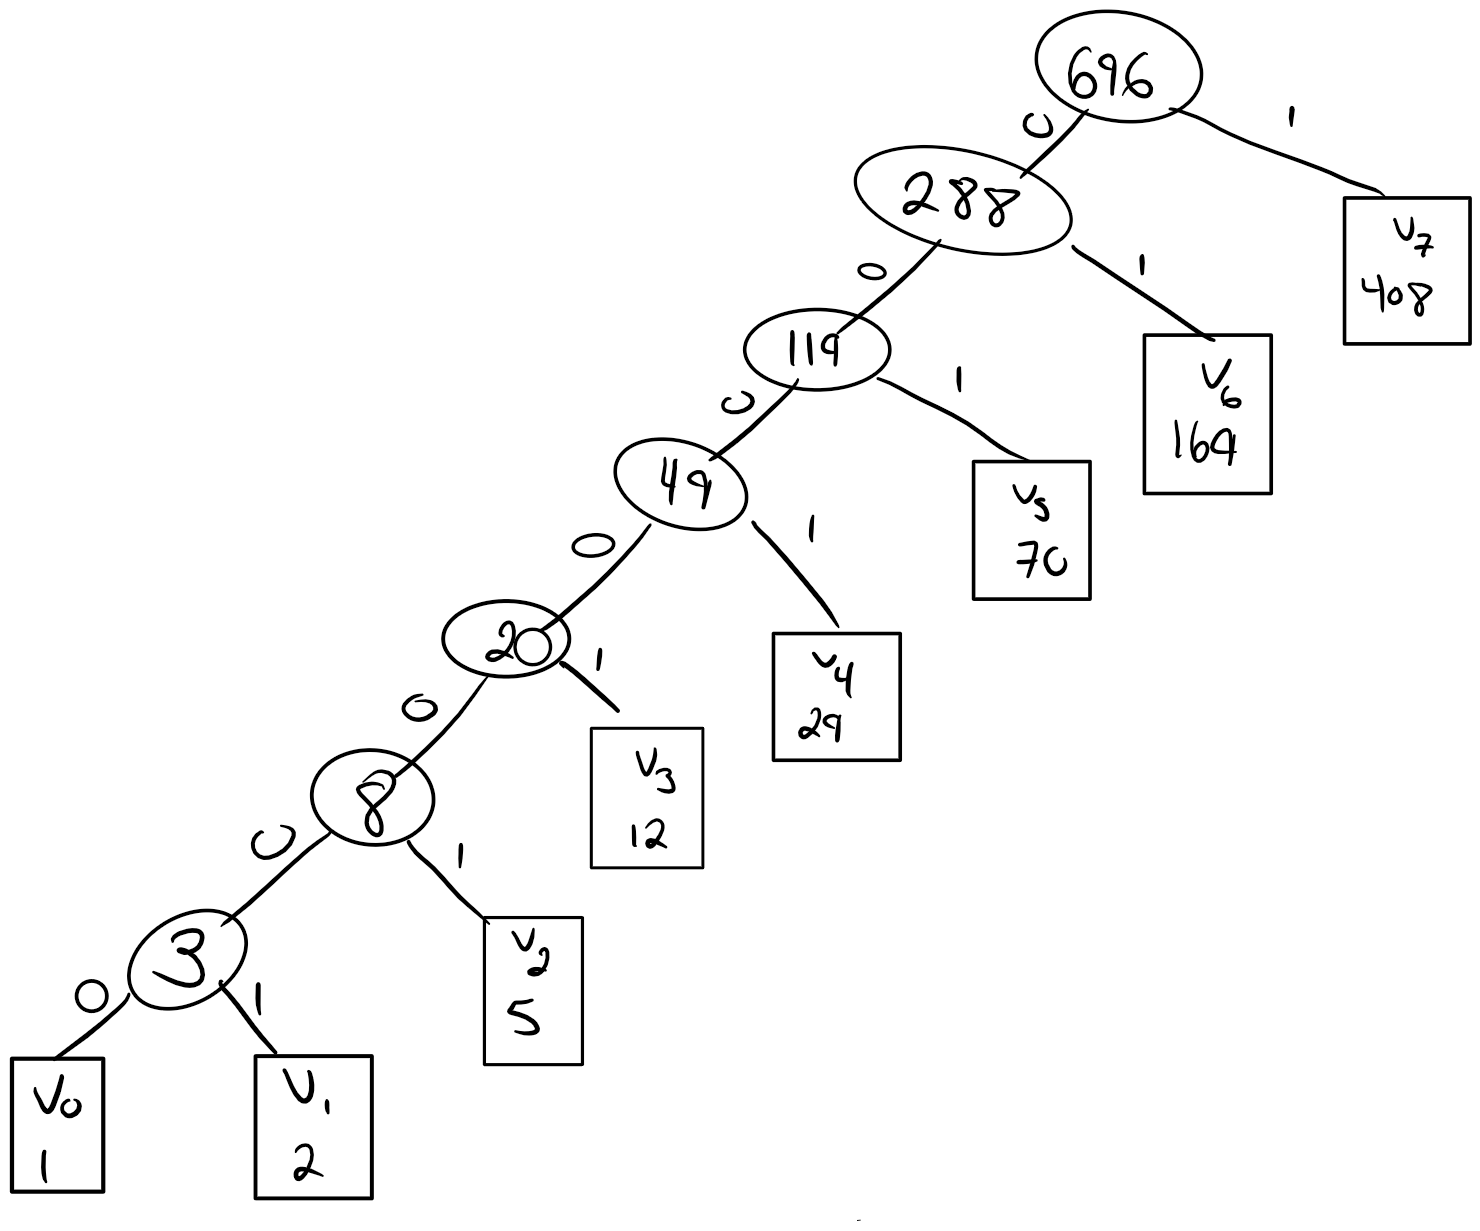
\includegraphics[scale=0.6]{PS5bQ3.png} 
\end{solution}
\pagebreak


\item (5 pts) Assume you run your Huffman tree algorithm and you produce the following pre-fix codes. Describe why there must be an error in your algorithm.
\begin{verbatim}
    S = 00
    c = 01
    i = 001
    e = 011
    n = 101
\end{verbatim}
\begin{solution}
This cannot be a valid Huffman code because Huffman codes are prefix codes. The algorithm must have an error in it because no code can be a prefix for another, and S is a prefix for c, i, and e and c is a prefix for e, etc.
\end{solution}
\pagebreak

\item (10 pts) Assume you're given an integer matrix that represents a plot of land, where the value at that location in the matrix represents the height above sea level. A value of zero indicates water. A pond is a region of water connected vertically, horizontally, or diagonally. The size of the pond is the total number of connected water cells. Write an algorithm to compute the sizes of all ponds in the matrix.

Example:
\begin{verbatim}
    0 2 1 0
    0 1 0 1
    1 1 0 1
    0 1 0 1
\end{verbatim}

would output 1, 2, 4.
\begin{enumerate}
    \item (3 pts) Describe the graph data structure that your algorithm will use for this problem.
    
    \begin{solution}
For this problem, the graph will be an undirected graph where all verticies have edges to all of the verticies that are adjacent to it. For example, if the 0 in the top left hand corner is s, it would have edges from $s-0$, $s-2$, $s-1$. 
    \end{solution}
\pagebreak
    
    \item (2 pts) Provide a 3-4 sentence description of how your algorithm works, including how the matrix is converted to the graph, how adjacent vertices are identified, and how the algorithm traverses the graph to identify connected vertices.
    
    \begin{solution}
This algorithm will go through each vertex in the graph and check if the value of the vertex is 0. If not, it will move on to the next. For each vertex equal to zero, it will iterate through it's adjacent verticies and select edges where the adjacent vertex is 0 and increment the count of the size of that pond. It will then mark the vertex as visted and move on to the next vertex with value 0, or move on to the next.
    \end{solution}
    
    \item (5 pts) Write an algorithm to solve this problem. 
    
    \begin{solution}Pseudocode:
\begin{verbatim} 
def selectPonds(G):
   lengths = []
   length = 0
   for each vertex in G: // Add edges between all adjacent verticies
      for adjVertex in vertex.adj:
         if adjVertex == 0:
            length += 1
         else:
            lengths.append(length)
   
         
   
\end{verbatim}
    \end{solution}
    
\end{enumerate}


\end{enumerate}

\end{document}
